\section{Experiments}\label{sec::dcme_experiments}

We conduct experiments on tasks of text classification and word embedding,
evaluating the proposed DCME approach by examining its computational and
learning efficiency. For comparison, we implement two sampling-based approaches,
noise contrastive estimation~(NCE) and negative sampling~(NS), as well as the
maximum likelihood estimation using gradient descent~(GD). In order for DCME and
the sampling-based approaches to have comparable training speed, we set both the
cluster number $K$ of DCME and the sampling number of NCE and NS to 20, and also
control the interval between offline updates in DCME with $\beta = 1$. Two
variants of DCME, DCME-Q0 and DCME-Q10, are developed, the latter of which
applies the online/offline tuning with $Q=10$. All the algorithms are run with
20 threads in parallel on a 64-bit Linux machine with the Intel Xeon 3.60GHz CPU
(20 core). Our code is implemented in C and available for download at:
\url{https://www.dropbox.com/s/e6b3fj2w0lq6jbt/code.tar.gz}

\begin{figure*}
  \centering
        \begin{subfigure}[h]{0.7\textwidth}
            \centering
            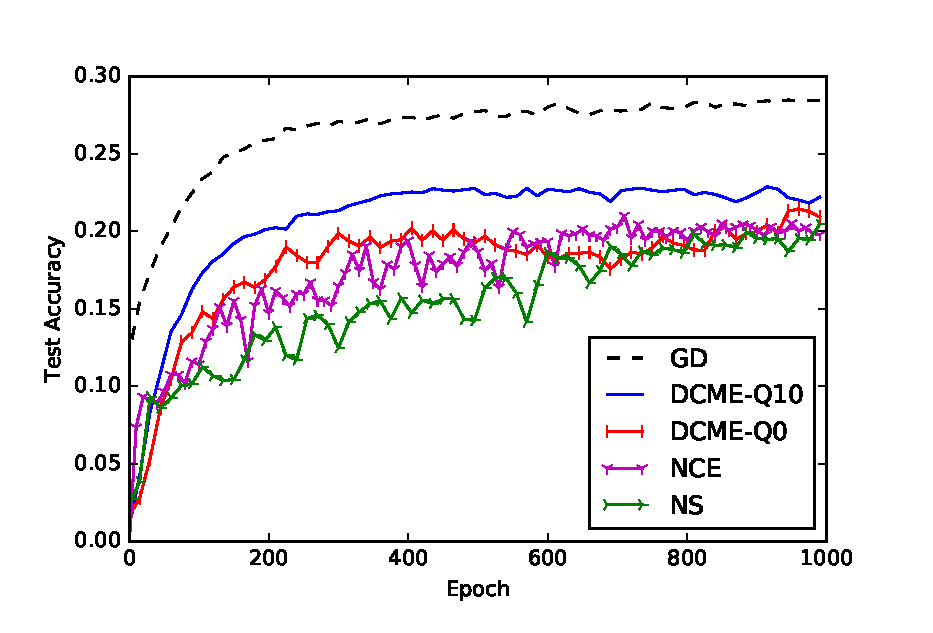
\includegraphics[width=\linewidth]{dcme/classification.eps}
            \captionsetup{justification=centering}
            \caption{Comparison of Test Accuracy for Classification\\
              Trained on ACM Digital Library Dataset}
            \label{fig::classification}
        \end{subfigure}
        \hfill
        \begin{subfigure}[h]{0.7\textwidth}
            \centering
            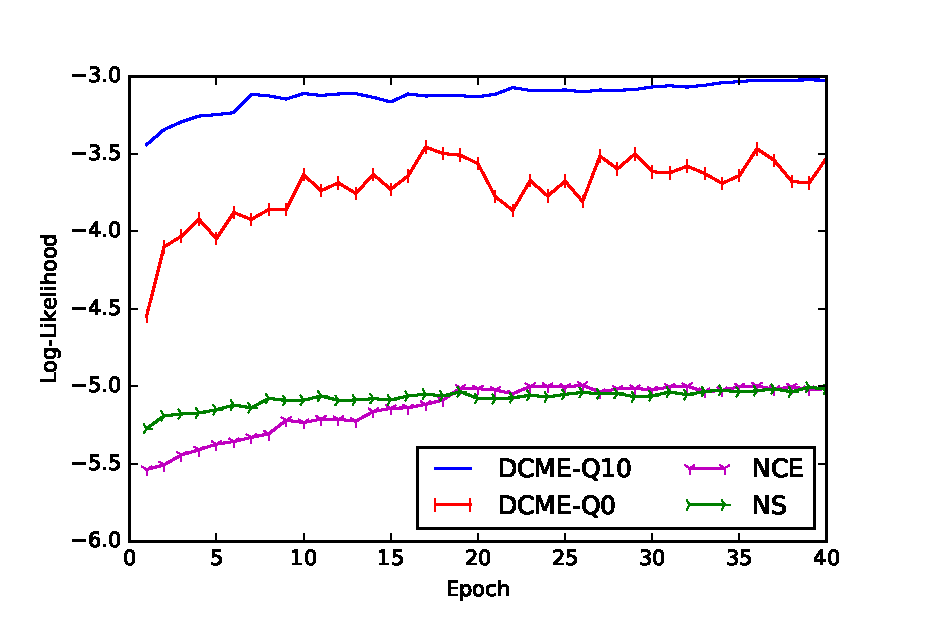
\includegraphics[width=\linewidth]{dcme/word_embedding.eps}
            \captionsetup{justification=centering}
            \caption{Comparison of Log-Likelihood for Embedding \\
              Trained on NYT Dataset}
            \label{fig::word_embedding}
        \end{subfigure}
        \begin{subfigure}[h]{0.65\textwidth}
            \centering
            \begin{tabular}{c|c|c|c|c}
              DCME-Q10  & DCME-Q0   & NCE   & NS        & GD     \\ \hline\hline
              9.50      & 7.94      & 6.21  & 6.16      & 165.91 \\
            \end{tabular}
            \captionsetup{justification=centering}
            \caption{Time Cost (Second) per Epoch in Classification}
            \label{tab::classification_time}
        \end{subfigure}
        \begin{subfigure}[h]{0.65\textwidth}
            \centering
            \begin{tabular}{c|c|c|c}
              DCME-Q10  & DCME-Q0   & NCE     & NS       \\ \hline\hline
              33.49     & 25.59     & 22.22   & 20.80    \\
            \end{tabular}
            \captionsetup{justification=centering}
            \caption{Time Cost (Minute) per Epoch in Embedding}
            \label{tab::we_time}
        \end{subfigure}
        \caption{ Performance on Text Classification and Word Embedding }
\end{figure*}

\subsection{Evaluation on Text Classification}

We employ the ME model to predict the publishing venue of research papers using
the abstract. A public dataset ACM Digital Library is investigated. It has
$162,460$ papers published at $1,236$ conferences. We hold out $10\%$ of the
documents for testing. Each paper is represented by the word count features of
the top $30,000$ frequent words.

\Cref{fig::classification} shows the learning curves of algorithms trained
at each epoch, and \Cref{tab::classification_time} reports the training
speed. It is clear that GD does not scale well to large number (thousands or
more) of items. DCME is 17-20 times faster than GD while the ratio is around 26
for sampling-based approaches. But it does give an estimation about the
upper-bound performance by leveraging the exact gradient information.  The curve
of GD converges in the least number of iterations while the test accuracy is the
highest.

DCME, on the other hand, achieves a computational efficiency similar to that of
the sampling-based approaches, but the accuracy is considerably higher.
Particularly, \Cref{fig::classification} validates that DCME benefits from
tuning the computation between online and offline updates. When $Q=10$, more
model parameters are updated online and there is thus less delay than that of
DCME-Q0. We also note that NCE and NS produce larger variances, which is
expected due to their sampling nature.

\subsection{Evaluation on Word Embedding}

For the word embedding task, we explore the New York Times (NYT) corpus from the
English Gigaword (Fifth Edition). It has a total of 1.35 billion words with
10.84 million unique terms. We retain the top 1 million frequent terms in the
vocabulary. To assess the performance, a randomly sampled \SI{1e-4} of the text
is withheld for testing. We train the word embeddings using CBOW with a context
window size of 10 and embedding dimensionality of 100.

We plot the test set average log-likelihood of each epoch in
\Cref{fig::word_embedding}, and report the time-per-epoch statistics in
\Cref{tab::we_time}. We do not evaluate GD in word embedding as it takes more
than days to run one epoch. The time costs for other algorithms are similar. The
results show that DCME remarkably outperforms NCE and NS.  However, DCME-Q0
exhibits a large performance variance. One possible explanation is as follows.
For $N$ as large as 1 million, the interval between offline updates is so long
that it creates two undesirable effects: (1) The delay results in a biased model
which contributes to a large training error; (2) The offline computation changes
the model drastically, as measured by the norm of the model difference, causing
inconsistency when another thread accesses the model while the offline update is
still in progress\footnote{The model parameters are shared by all threads and
  there is no mutex locks on writing to the model, which is a common practice
for efficiency in implementations including word2vec
  (\url{https://code.google.com/p/word2vec/}) and ours.}. For DCME-Q10, minimal
  variance is observed. Indeed, it offers the best trade-off between learning
  and computational efficiency.

\begin{table}[h]
  \centering
  \begin{tabular}{c||l|l|l}
    Model     & Semantic          & Syntactic         & Overall          \\
    \hline\hline
    DCME-Q10  & $\mathbf{-8.676}$ & $-8.648$          & $\mathbf{-8.654}$ \\
    DCME-Q0   & $-8.712$          & $\mathbf{-8.647}$ & $-8.663$          \\
    NCE       & $-8.784$          & $-8.782$          & $-8.783$          \\
    NS        & $-8.765$          & $-8.679$          & $-8.699$          \\
  \end{tabular}
  \captionsetup{justification=centering}
  \caption{Log-Likelihood on Semantic-Syntactic Word Relationship Dataset}
  \label{tab::we_analogy}
\end{table}

To assess the quality of the trained embeddings, we use the word analogy task,
which examines whether the embeddings learn the semantic/syntactic relationships
of words. For instance, the question which word is similar to ``small'' in the
same sense as ``biggest'' to ``big'' can be solved by predicting the target word
with a context vector $\vh_{biggest} - \vh_{big} + \vh_{small}$. We evaluate the
trained word embeddings after 15 epochs. And the results on the
Semantic-Syntactic Word Relationship test set~\cite{mikolov2013efficient} are
summarized in \Cref{tab::we_analogy}, where the best performance is highlighted
in bold. Again, it confirms that DCME achieves better model quality than
sampling-based NCE and NS.

% since they represent the main state of the art methods that can work efficiently with large numbers of items for ME.

% 0.017287 %   Semantic accuracy: 0.016449 %   Syntactic accuracy: 0.017556 %
% 0.017426 %   Semantic accuracy: 0.017061 %   Syntactic accuracy: 0.017543 %
% 0.016231 %   Semantic accuracy: 0.015777 %   Syntactic accuracy: 0.016377 %
% w2v
% 0.016666 %   Semantic accuracy: 0.015606 %   Syntactic accuracy: 0.017006 %
% 0.015336 %   Semantic accuracy: 0.015305 %   Syntactic accuracy: 0.015346 %
% 0.015792 %   Semantic accuracy: 0.015731 %   Syntactic accuracy: 0.015811 %
